% Written by Anders Sjoqvist and Ulf Lundstrom, 2009
% The main sources are: tinyKACTL, Beta and Wikipedia

\chapter{Mathematics}

\section{Equations}
In general, given an equation $Ax = b$, the solution to a variable $x_i$ is given by
\[x_i = \frac{\det A_i'}{\det A} \]
where $A_i'$ is $A$ with the $i$'th column replaced by $b$.

\section{Geometry}

\subsection{Triangles}
Side lengths: $a,b,c$\\
Semiperimeter: $p=\dfrac{a+b+c}{2}$\\
Area: $A=\sqrt{p(p-a)(p-b)(p-c)}$\\
Circumradius: $R=\dfrac{abc}{4A}$\\
Inradius: $r=\dfrac{A}{p}$\\
Length of median (divides triangle into two equal-area triangles): $m_a=\tfrac{1}{2}\sqrt{2b^2+2c^2-a^2}$\\
Length of bisector (divides angles in two): $s_a=\sqrt{bc\left[1-\left(\dfrac{a}{b+c}\right)^2\right]}$\\
Law of sines: $\dfrac{\sin\alpha}{a}=\dfrac{\sin\beta}{b}=\dfrac{\sin\gamma}{c}=\dfrac{1}{2R}$\\
Law of cosines: $a^2=b^2+c^2-2bc\cos\alpha$\\
Law of tangents: $\dfrac{a+b}{a-b}=\dfrac{\tan\dfrac{\alpha+\beta}{2}}{\tan\dfrac{\alpha-\beta}{2}}$\\

\subsection{Quadrilaterals}
With side lengths $a,b,c,d$, diagonals $e, f$, diagonals angle $\theta$, area $A$ and
magic flux $F=b^2+d^2-a^2-c^2$:

\[ 4A = 2ef \cdot \sin\theta = F\tan\theta = \sqrt{4e^2f^2-F^2} \]

 For cyclic quadrilaterals the sum of opposite angles is $180^\circ$,
$ef = ac + bd$, and $A = \sqrt{(p-a)(p-b)(p-c)(p-d)}$.

%% \subsection{Spherical coordinates}
%% \begin{center}
%% 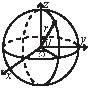
\includegraphics[width=25mm]{content/math/sphericalCoordinates}
%% \end{center}

\section{Markov chains}
A \emph{Markov chain} is a discrete random process with the property that the next state depends only on the current state.
Let $X_1,X_2,\ldots$ be a sequence of random variables generated by the Markov process.
Then there is a transition matrix $\mathbf{P} = (p_{ij})$, with $p_{ij} = \Pr(X_n = i | X_{n-1} = j)$,
and $\mathbf{p}^{(n)} = \mathbf P^n \mathbf p^{(0)}$ is the probability distribution for $X_n$ (i.e., $p^{(n)}_i = \Pr(X_n = i)$),
where $\mathbf{p}^{(0)}$ is the initial distribution.

% \subsubsection{Stationary distribution}
$\mathbf{\pi}$ is a stationary distribution if $\mathbf{\pi} = \mathbf{\pi P}$.
If the Markov chain is \emph{irreducible} (it is possible to get to any state from any state),
then $\pi_i = \frac{1}{\mathbb{E}(T_i)}$ where $\mathbb{E}(T_i)$  is the expected time between two visits in state $i$.
$\pi_j/\pi_i$ is the expected number of visits in state $j$ between two visits in state $i$.

For a connected, undirected and non-bipartite graph, where the transition probability is uniform among all neighbors, $\pi_i$ is proportional to node $i$'s degree.

% \subsubsection{Ergodicity}
A Markov chain is \emph{ergodic} if the asymptotic distribution is independent of the initial distribution.
A finite Markov chain is ergodic iff it is irreducible and \emph{aperiodic} (i.e., the gcd of cycle lengths is 1).
$\lim_{k\rightarrow\infty}\mathbf{P}^k = \mathbf{1}\pi$.

% \subsubsection{Absorption}
A Markov chain is an A-chain if the states can be partitioned into two sets $\mathbf{A}$ and $\mathbf{G}$, such that all states in $\mathbf{A}$ are absorbing ($p_{ii}=1$), and all states in $\mathbf{G}$ leads to an absorbing state in $\mathbf{A}$.
The probability for absorption in state $i\in\mathbf{A}$, when the initial state is $j$, is $a_{ij} = p_{ij}+\sum_{k\in\mathbf{G}} a_{ik}p_{kj}$.
The expected time until absorption, when the initial state is $i$, is $t_i = 1+\sum_{k\in\mathbf{G}}p_{ki}t_k$.
